\subsection{Kernels and Filters}
\begin{frame}{}
    \LARGE CNN Hyperparameter: \textbf{Kernels and Filters}
\end{frame}

\begin{frame}[allowframebreaks]{Kernels and Filters}
    \begin{itemize}
        \item Kernels and filters are the same thing in CNNs.
        \item They are small matrices used to extract features from input data.
        \item The kernel \textbf{slides over} the input image, performing \textbf{element-wise} multiplication and summation.
        \item This process is known as \textbf{convolution}.
    \end{itemize}

    \framebreak

    \begin{figure}
        \centering
        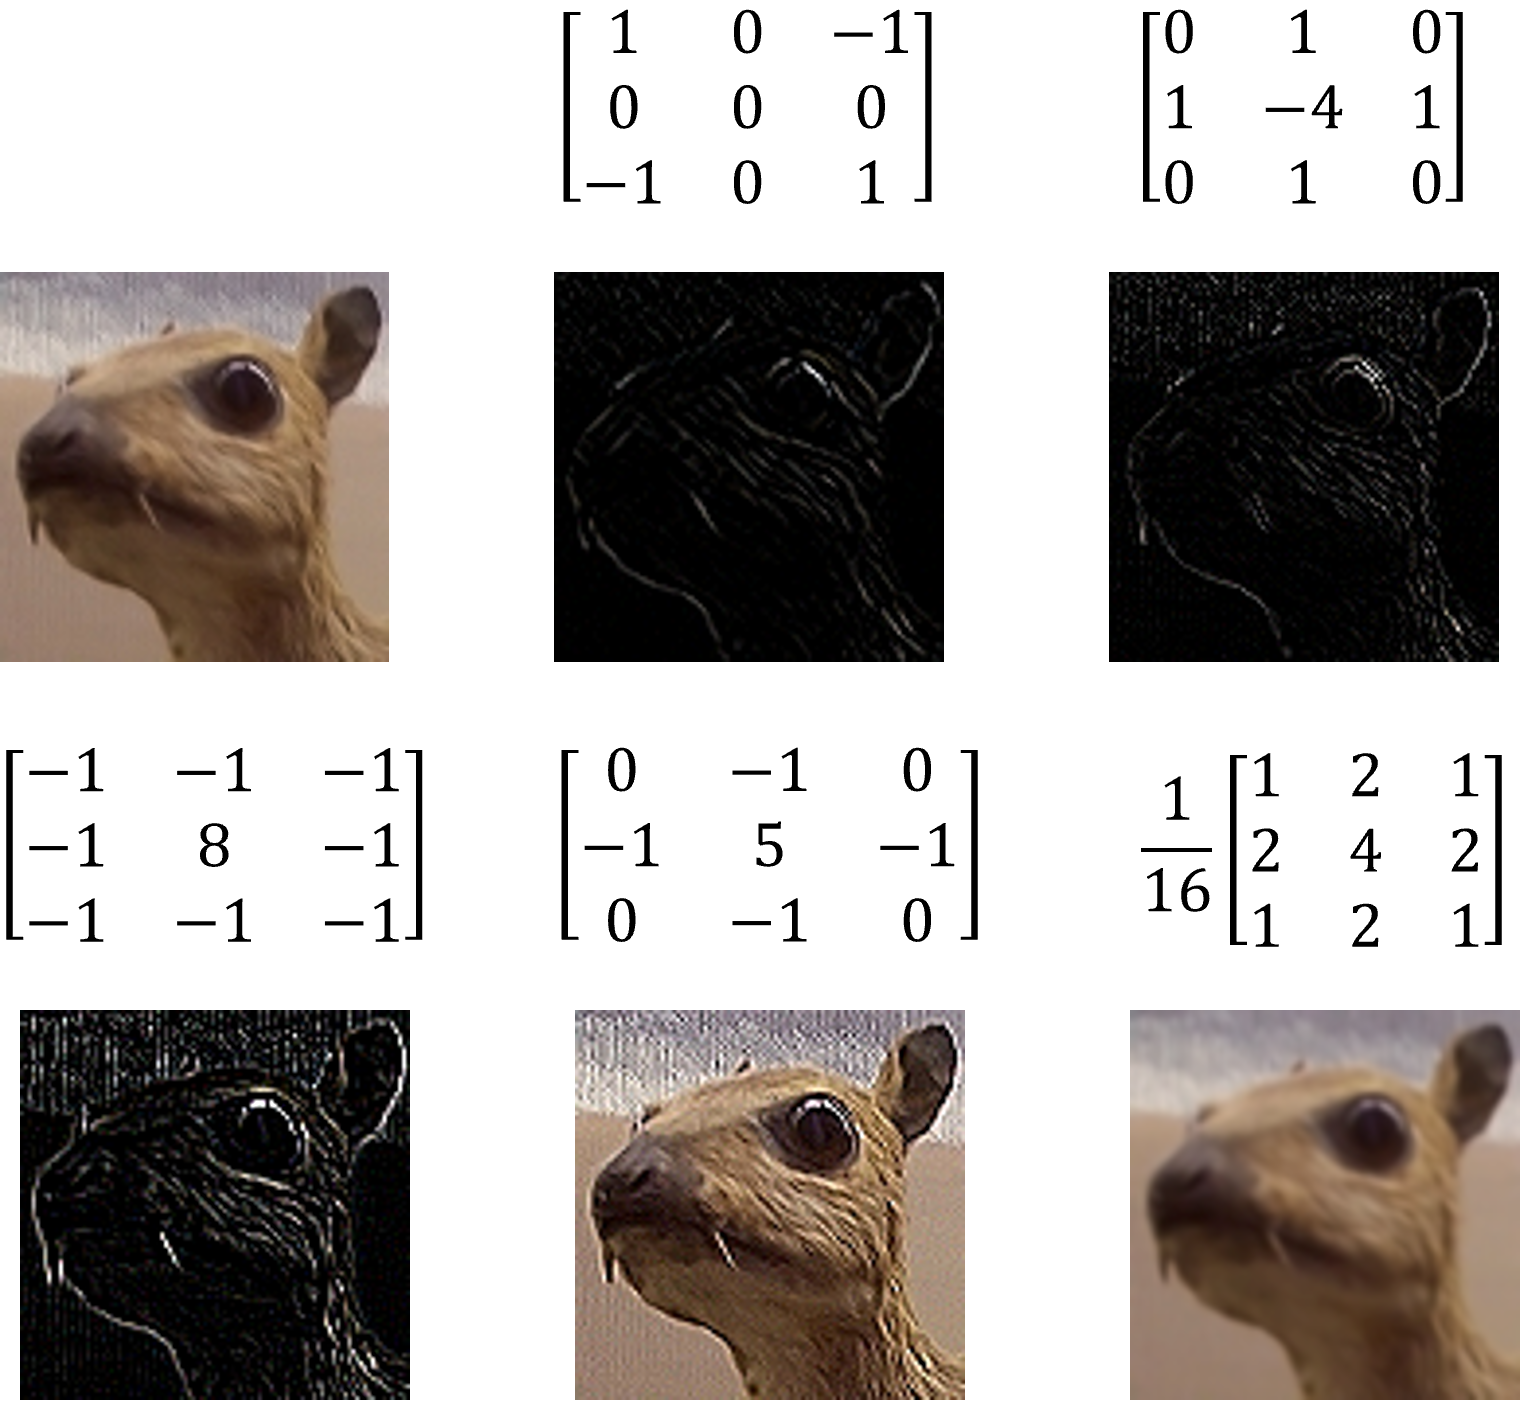
\includegraphics[width=1.0\textwidth,height=0.9\textheight,keepaspectratio]{images/cnn/conv_12.png}
    \end{figure}

    \framebreak
    \begin{itemize}
        \item The kernel size is typically smaller than the input image (e.g., 3x3, 5x5).
        \item Multiple kernels can be used in a single convolutional layer to extract different features.
        \item Each kernel produces a feature map, which is a transformed version of the input image highlighting specific features.
        \item The number of filters (kernels) in a layer determines the depth of the output feature map.
    \end{itemize}
\end{frame}